\section{Часть 3 — Эксперименты и результаты}

\begin{frame}{Датасет и постановка эксперимента}
Оценка проводится на бенчмарке \textbf{PISA} для Isabelle/HOL:
\begin{itemize}
  \item корпус теорем и доказательств из Isabelle + Archive of Formal Proofs;
  \item тестовый набор: \textbf{6336} теорем.
\end{itemize}

\vspace{2mm}
Меряем долю теорем, доказанных полностью автоматически.
\end{frame}

\begin{frame}{Вопросы исследования}
\begin{enumerate}
  \item Насколько LLM эффективны в генерации \textbf{целых} доказательств?
  \item Можно ли улучшить результат через \textbf{repair} по ошибкам Isabelle?
  \item Помогает ли \textbf{контекст} из файла теории?
  \item Влияет ли \textbf{размер} модели?
  \item Как Baldur соотносится с state-of-the-art методами (например, Thor)?
\end{enumerate}
\end{frame}


\begin{frame}{Экспериментальные результаты}
\centering
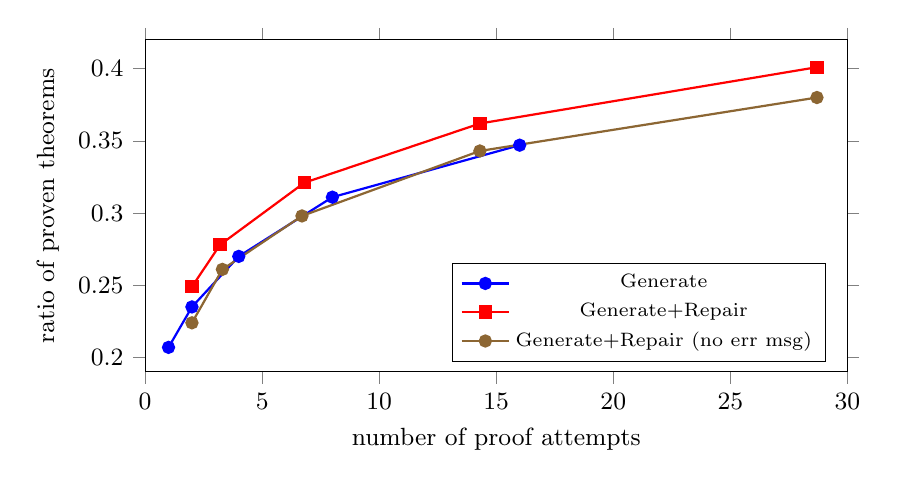
\begin{tikzpicture}
\begin{axis}[
    width=10.5cm,
    height=5.8cm,
    xmin=0, xmax=30,
    ymin=0.19, ymax=0.42,
    xlabel={number of proof attempts},
    ylabel={ratio of proven theorems},
    xtick={0,5,10,15,20,25,30},
    ytick={0.20,0.25,0.30,0.35,0.40},
    legend style={
        at={(0.97,0.03)},
        anchor=south east,
        draw=black,
        fill=white,
        font=\scriptsize
    },
    label style={font=\small},
    tick label style={font=\small},
    tick align=outside,
]

\addplot[color=blue, mark=*, thick] coordinates {
    (1,0.207)
    (2,0.235)
    (4,0.270)
    (8,0.311)
    (16,0.347)
};
\addlegendentry{Generate}

\addplot[color=red, mark=square*, thick] coordinates {
    (2,0.249)
    (3.2,0.278)
    (6.8,0.321)
    (14.3,0.362)
    (28.7,0.401)
};
\addlegendentry{Generate+Repair}

\addplot[color={rgb,1:red,0.55;green,0.40;blue,0.20}, mark=*, thick] coordinates {
    (2,0.224)
    (3.3,0.261)
    (6.7,0.298)
    (14.3,0.343)
    (28.7,0.380)
};
\addlegendentry{Generate+Repair (no err msg)}

\end{axis}
\end{tikzpicture}

\vspace{0.2cm}
{\small Ratio of theorems proven vs inference cost}
\end{frame}

\begin{frame}{Статистика по разным моделям}
\centering
\small

\begin{tabular}{lcc}
\toprule
Model & 16 samples & 64 samples \\
\midrule
Baldur 8b generate & 34.8\% & 40.7\% \\
Baldur 8b generate + repair & 36.3\%$^{*}$ & --- \\
Baldur 8b w/ context & 40.9\% & 47.5\% \\
Baldur 62b w/ context & 42.2\% & 47.9\% \\
\midrule
Baldur 8b w/ context $\cup$ Thor & --- & 65.7\% \\
\bottomrule
\end{tabular}

\vspace{0.3cm}
{\tiny $^{*}$Repair uses half the samples and one repair attempt per sample.}
\end{frame}

\begin{frame}{Статистика доказательств с использованием контекста}
\centering

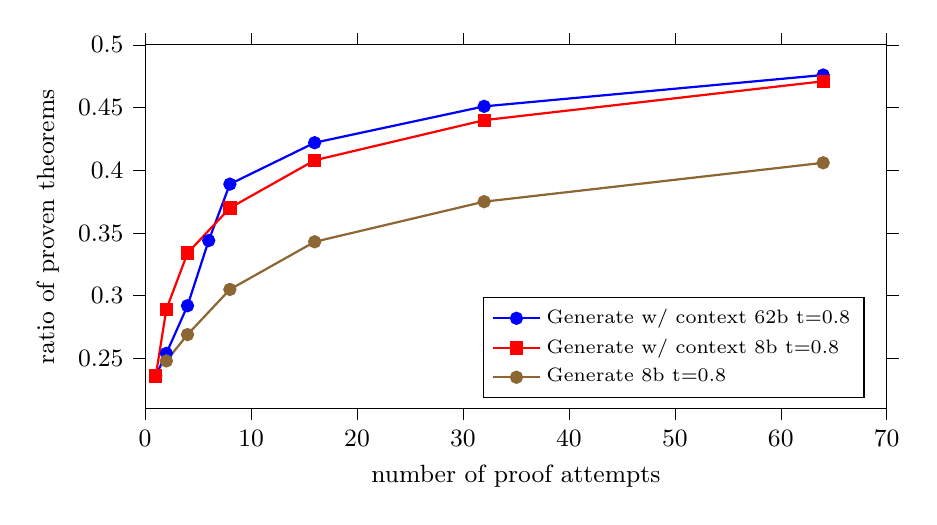
\begin{tikzpicture}
\begin{axis}[
    width=11cm,
    height=6.2cm,
    xmin=0, xmax=70,
    ymin=0.21, ymax=0.50,
    xlabel={number of proof attempts},
    ylabel={ratio of proven theorems},
    xtick={0,10,20,30,40,50,60,70},
    ytick={0.25,0.30,0.35,0.40,0.45,0.50},
    tick align=outside,
    axis line style={black},
    tick style={black},
    label style={font=\small},
    tick label style={font=\small},
    legend style={
        at={(0.97,0.03)},
        anchor=south east,
        draw=black,
        fill=white,
        font=\scriptsize,
        legend cell align=left
    }
]

% Generate w/ context 62b t=0.8
\addplot[
    color=blue,
    mark=*,
    thick
] coordinates {
    (1,0.236)
    (2,0.254)
    (4,0.292)
    (6,0.344)
    (8,0.389)
    (16,0.422)
    (32,0.451)
    (64,0.476)
};
\addlegendentry{Generate w/ context 62b t=0.8}

% Generate w/ context 8b t=0.8
\addplot[
    color=red,
    mark=square*,
    thick
] coordinates {
    (1,0.236)
    (2,0.289)
    (4,0.334)
    (8,0.370)
    (16,0.408)
    (32,0.440)
    (64,0.471)
};
\addlegendentry{Generate w/ context 8b t=0.8}

% Generate 8b t=0.8
\addplot[
    color={rgb,1:red,0.55;green,0.40;blue,0.20},
    mark=*,
    thick
] coordinates {
    (2,0.248)
    (4,0.269)
    (8,0.305)
    (16,0.343)
    (32,0.375)
    (64,0.406)
};
\addlegendentry{Generate 8b t=0.8}

\end{axis}
\end{tikzpicture}

\vspace{0.2cm}
{\small Ratio of theorems proven vs.\ inference cost for models with different sizes and temperatures.}
\end{frame}

\begin{frame}{Комплементарность с Thor}
\textbf{Thor} использует комбинацию:
\begin{itemize}
  \item модели;
  \item поиска;
  \item \textbf{Sledgehammer} (premise selection/автоматические решатели).
\end{itemize}

\begin{frame}{Итоги по эффективности (по тексту статьи)}
Ключевые выводы, которые выносим в доклад:
\begin{itemize}
  \item Baldur доказывает заметную долю теорем автоматически (порядка \(\sim 40\%\)).
  \item Repair даёт прирост и важен именно благодаря \textbf{error messages} (сообщениям с ошибками).
  \item Контекст из theory-файла повышает успешность (порядка \(\sim 47\%\)).
  \item Более крупные модели работают лучше.
\end{itemize}
\end{frame}

\vspace{2mm}
Наблюдение статьи:
\begin{itemize}
  \item Baldur и Thor решают \textbf{частично разные} теоремы;
  \item объединение результатов даёт около \textbf{65.7\%} доказанных теорем.
\end{itemize}
\end{frame}

\begin{frame}[fragile]{Мини-идея premise selection (почему Thor силён)}
\lstset{style=code, language=}
\begin{lstlisting}
have "goal"
  by (smt lemma1 lemma2 lemma3)
\end{lstlisting}

Комментарий:
\begin{itemize}
  \item успех автоматического решателя зависит от выбора нужных лемм;
  \item Thor активно использует такие механизмы через Sledgehammer.
\end{itemize}
\end{frame}

\begin{frame}{Главные выводы}
\begin{itemize}
  \item LLM могут генерировать \textbf{полные} формальные доказательства.
  \item Error messages из proof assistant — полезный сигнал для \textbf{proof repair}.
  \item Whole-proof подход упрощает архитектуру по сравнению с step-by-step search.
  \item В перспективе: комбинировать подходы (LLM + search/premise selection).
\end{itemize}
\end{frame}